\section{Experiments}

\paragraph{A metric to determine when MTL performs better STL.}
\begin{table}
\begin{center}
  \begin{tabular}{c c c c c}
  \toprule
    \multirow{2}{*}{{\bf Threshold}}  & \multicolumn{2}{c}{{\bf Text classification}} & \multicolumn{2}{c}{{\bf ChestX-ray14}} \\
    & Precision &  Recall & Precision &  Recall \\
    \cmidrule(lr){1-1} \cmidrule(lr){2-3} \cmidrule(lr){4-5}
    0.0 & 0.596 & 1.000 & 0.593 & 1.000 \\
    0.1 & 0.756 & 0.388 & 0.738 & 0.462 \\
    0.2 & 0.919 & 0.065 & 0.875 & 0.044 \\	
    0.3 & 1.000 & 0.004 &     - &     - \\
  \bottomrule
  \end{tabular}
\end{center}
\caption{Ablation study on when should use MTL via different source/target task accuracy. Note: For text classification tasks, the source task training data size ranges from 500 to 1,500 and target task training data size is 1000; For ChestX-ray14, the training data size is 10,000.}
\label{tab:mtl_better_than_stl}
\end{table}

\paragraph{When should we align task covariances in MTL.}
\begin{figure}
	\centering
	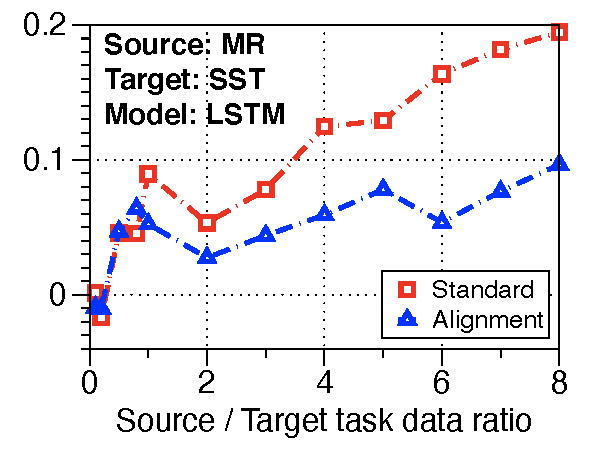
\includegraphics[width=0.5\textwidth]{figures/ratio_alignment_mr_sst_lstm.pdf}
	\caption{Covariate shift experiment.}
\end{figure}

\begin{figure}
	\centering
	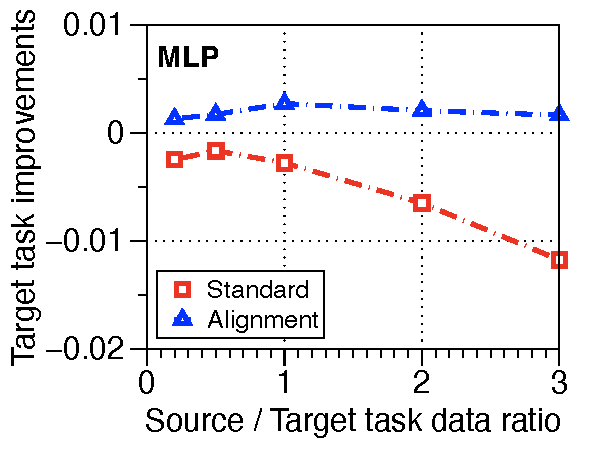
\includegraphics[width=0.5\textwidth]{figures/ratio_alignment_mlp.pdf}
	\caption{Covariate shift experiment.}
\end{figure}
